
\section{Introduction}

A large amount of electronic components exist in aircrafts, satellites, and cars, many of which perform increasingly critical roles autonomously.  This trend of autonomous vehicles will continue to grow for the foreseeable future, such as the growth of self-driving cars and UAVs many of which utilize all electric powertrains.

Understanding the behavior of components over its lifetime must be developed to monitor the health of these components.  Of particular note to prognostics is the capability to anticipate failures and predict the remaining life of these components.  This allows maintenance and part replacement to be planned optimally, the fixing of components before they fail, and allow aircrafts to optimally plan missions.

Due to the safety management, estimating the remaining useful life (RUL) of \lib batteries has become a challenging problem in the fields of reliability, automatic test, power sources, and electric vehicles, etc. 

This problem can be broken into two parts: 
\begin{enumerate}
\item building a model that can accurately estimate the future state of the electrical component
\item creating an alarm system that triggers before said component is estimated to fail.  
\end{enumerate}
The accuracy of the model’s estimates directly impact the effectiveness of the alarm system.

Prior research has been performed in this field where a system was presumed to be a linear dynamic system specified in discrete time.  A dynamic Bayes network (DBN) was used to model the linear dynamic system (LDS) to predict future output of a selected feature of the component.  An optimal alarm system was then constructed where the alarm would trigger if the conditional probability of a critical event was above a certain threshold probability.

This paper focuses entirely on on two different machine learning approaches, created in \MATLAB, to model a specific electrical component, a 18650 \lib battery, using a large dataset of experimental measurements recorded by NASA.



The rest of the document is organized as follows: Section 2 presents recent related work and studies on Predictive Models for \lib  batteries. The problem description and the addressed challenges are explained in Section 3. Our approach is presented in Section 4. Subsequently, the evaluation results are discussed in Section 5. We conclude with a view on future work in Section 6.

\section{Related Work}
At present, the various approaches of battery State of Charge (SOC) estimation and RUL prediction can be generally classified into two categories \cite{Liu:2014:LBR:2662603.2662621}: statistical data-driven and model based \cite{ZHANG20116007}, \cite{Si2011RemainingUL}. There are lots of research work focusing on performance degradation, SOC assessment, RUL estimation for the \lib battery
\cite{Bhaskar01}, \cite{4579269}, \cite{zio:hal-00609502}. Especially for the
\lib battery prognostics, the prediction uncertainty, and
the applicability of the model-based and data-driven methods have always
been challenging problems in this area.

Lots of researchers such as Bhaskar Saha and Kai Goebel
and others researchers in the Prognostics Center of
Excellence (PCoE) of the NASA AMES Center achieved
the battery RUL prediction as well as the uncertainty
representation and management with particle filter (PF)
algorithm \cite{Bhaskar01}, \cite{4579269}. Moreover, the Artificial Neural
Networks (ANN) \cite{liu_2010}, Extended Kalman
Filter (EKF) \cite{1159187}, Support Vector Machine (SVM) \cite{4655607}, Relevance
Vector Machine (RVM) \cite{doi:10.1177/0142331208092030} and other machine
learning and statistical algorithms \cite{RICHARDSON2017209}, \cite{BRONDANI2017} are applied in \lib
battery prognostics. Finally, lots of physical
models, chemistry model and other related empirical model
are developed or applied in the battery RUL estimation \cite{FLEISCHER2014276}.

All of the RUL estimation frameworks have become an effective
and practical approach for \lib battery degradation
analysis and estimation. However, to obtain the model or to identify the
model parameters is very difficult in most cases due to complicated operating conditions. The main drawback is that these modeling approaches do not consider the varied operation condition for an on-line application, a fact that leads to sub-optimal results. On the
other hand, most of the data-driven prognostics algorithms
require high computing complexity even in the case of simple application, calling for more time-efficient techniques.

\section{Methodology}

\subsection{Dataset}

To evaluate the performance of two approaches analyzed in the following parts, we used a dataset provided by NASA\footnote{\url{https://ti.arc.nasa.gov/tech/dash/groups/pcoe/prognostic-data-repository/}} \cite{bole2014adaptation}. The dataset used was derived from a NASA experiment where a set of four 18650 \lib batteries, labeled from RW9 to RW12, were continuously operated using a sequence of charging and discharging currents between -4.5A and 4.5. This type of charging and discharging operation is referred to in the experiment as a random walk (RW) operation. Each of the loading periods last 5 minutes or whenever the voltage goes outside the range of 4.2V to 3.2V, and after 1500 periods (about 5 days) a series of reference charging and discharging cycles were performed in order to provide reference benchmarks for battery state health.

The dataset includes the relative time the measurements were taken from the start of the experiment along with the temperature, current, and voltage of the battery. Figures \ref{fig:first_50_rw} and \ref{fig:last_50_rw} show the measurements for voltage, current and temperature for the first and last 50 random walk cycles performed.

\begin{figure*}
\begin{multicols}{2}
	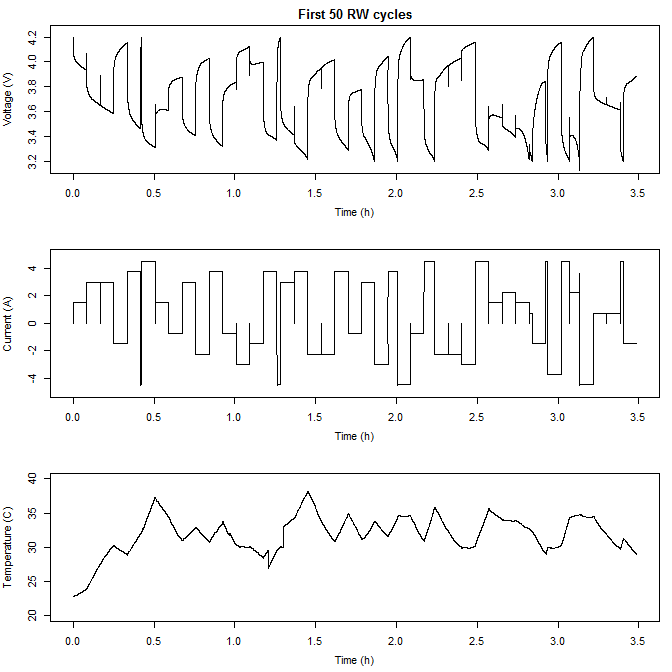
\includegraphics[height=2in, width=3.2in]{figures/GPR/first_50_rw}
	\caption{First 50 RW cycles of RW9}
	\label{fig:first_50_rw}
	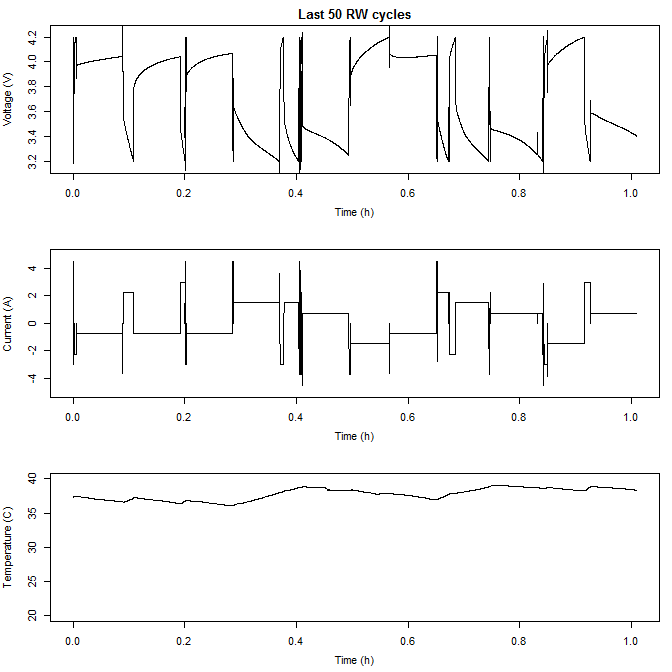
\includegraphics[height=2in, width=3.2in]{figures/GPR/last_50_rw}
	\caption{Last 50 RW cycles of RW10}
	\label{fig:last_50_rw}
\end{multicols}
\end{figure*}

Note that due to random nature of charging and discharging cycles performed during this experiment, the stable state preconditions required by the approach outlined in \cite{5571895} are violated and hence, non-linear methods should be adopted instead.

\subsubsection{Infrastructure} We used a machine with an Intel Core\textsuperscript{TM} i5-2557M Processor, 1.7 GHz, 4GB of RAM memory and \MATLAB, version R2017b.
\subsection{Gaussian Process Regression}

Gaussian process regression (GPR) is a statistical model where observations are continuous, such as time \cite{10.1371/journal.pone.0163004}.  The model is a powerful non-linear multivariate interpolation technique used in fields as far ranging as mining, remote sensing, and real estate appraisal. In machine learning, GPR models are nonparametric kernel-based probabilistic models that utilize lazy learning and a kernel function, which uses the similarity between points, to predict an unseen point in training data, along with the uncertainty of the prediction.

Observed values generally do not match the exact function values, but a noisy realization of them.  GPR models, which are probabilistic, are able to compute the prediction intervals using these observed values and predict all values between the observed values.  This means that, the model becomes more accurate as more observed values are given to the model as training data as it is easier to find the function that fits the data.  However, since GPR models are created through lazy learning, more data dramatically increases the time to train a model.  As an addendum, GPR model predictions have drastically increased error when predicting values outside of the time range that the training data is in, as the prediction interval bounds drastically increase due to the lack of observed values for future time.  Fortunately, in our case, our dataset includes observed data of the entire lifetime of the battery and so prediction intervals are expected to remain consistent.


In this paper, voltage was selected as the output of the GPR model, with time, temperature, and current as inputs.  Given the sheer size of data for a single battery, over 8 million data rows, and the limitation of \MATLAB, roughly 30 thousand data rows were randomly chosen over the entire RW9 dataset to be used as training data.  Multiple GPR models were trained using different kernel functions: rational quadratic, squared exponential, matern 5/2, and exponential.  Each model used 5-fold cross validation.  The best model was selected based on the lowest root mean square error (RMSE), the model that best fit the training data.  RW10 data was used as a test set for the trained model.  The models were created using \MATLAB\textquotesingle s Statistics and Machine Learning Toolbox\textsuperscript{TM}, as shown in Figure \ref{fig:regresion_learner}.

\begin{figure}
 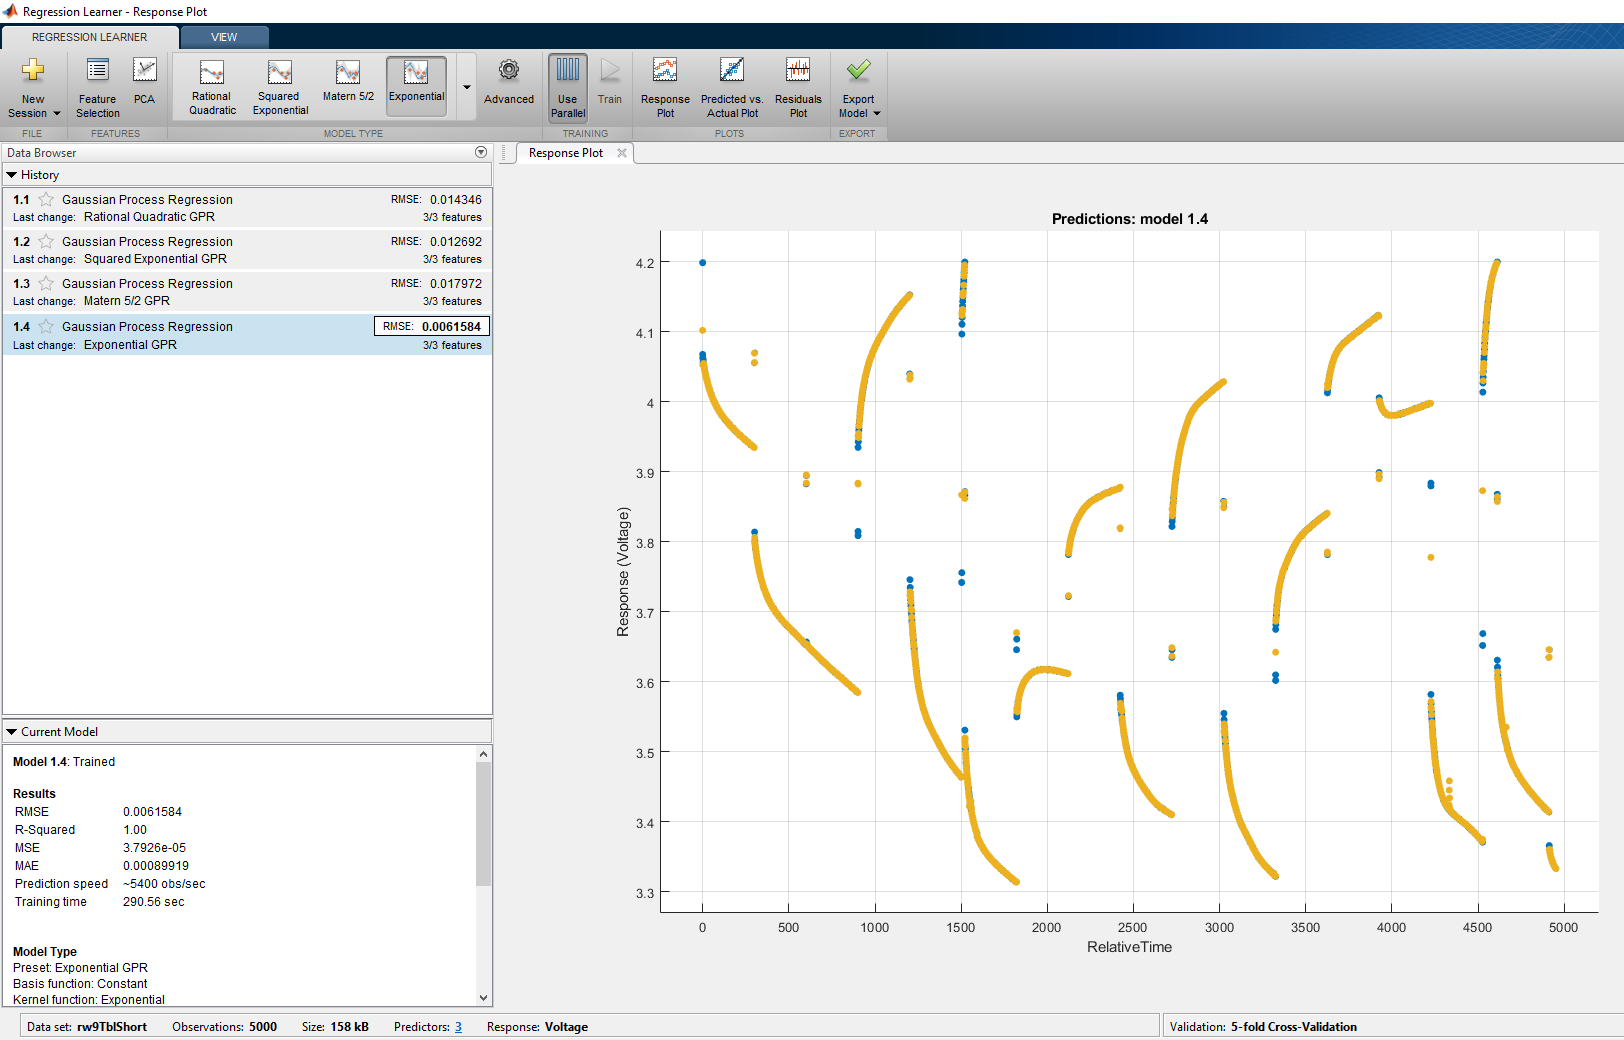
\includegraphics[height=2in, width=3in]{figures/GPR/regresion_learner}
\caption{\MATLAB\textquotesingle s Regression Learner used to find best fit GPR Model}
\label{fig:regresion_learner}
\end{figure}


\subsection{Battery Modeling Using Battery Equivalent Circuit}

In this approach, we can predict the state of the battery by modeling its physical characteristics. There are two important requirements that must be provided before the battery internal parameters are estimated. First, we need the battery equivalent circuit. This equivalent circuit later will be used to construct \MATLAB\'s Simscape \footnote{\url{https://www.mathworks.com/products/simscape.html}} and Simulink\footnote{\url{https://www.mathworks.com/products/simulink.html}} model. The second requirement is the real data from experiments performed on the battery. In this case, the dataset will be discharging data from RW9 dataset provided by NASA. Even though the dataset used in GPR experiment is still applied, in this approach, the total random walk cycles are not required for the parameter estimation. To construct the battery model and estimates its internal parameters, we only need the very first discharging cycle of the battery in the initial experiment since we only need the discharging data where the battery condition is still good and optimal so that we can the create a proper model for our experiment. By using these two requirements, parameter estimation will be performed in the Simulink Design Optimization tool provided by \MATLAB. The goal of this estimation is to estimate the internal parameter values of the battery, e.g. $R_0$, $R_1$, $C_1$, and $Em$.

\subsubsection{Battery Model}

In this project, we chose a first order $RC$ circuit as the equivalent circuit of the battery. This circuit consists of $Em$, $R_1$, $R_0$ and $C_1$, where $Em$ is the electromotive force from the voltage source, $R_0$ and $R_1$ is the resistor, and $C_1$ is the battery capacitance. This experiment could be conducted by using more than one RC component to obtain more accurate battery parameter results, however, since the focus of the paper is on the machine learning aspect, we refrained from additional complexity in the battery model.



In the model shown in Figure \ref{fig:circuit_RC}, $R_0$, $R_1$, $C_1$, and $Em$ are dependent on State of Charge (SOC) and battery temperature (T). Thus, these parameters will be 2D look-up tables that accept SOC and temperature as the matrix index. 

\begin{figure}
 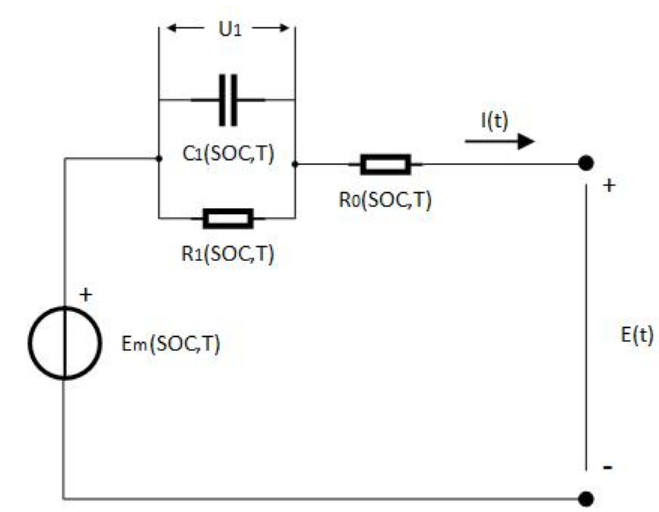
\includegraphics[height=1.5in, width=2in]{figures/Circuit_RC}
\caption{Equivalent circuit of battery using a first RC circuit}
\label{fig:circuit_RC}
\end{figure}



The dependency between each battery component with SOC and temperature should be reflected in the Simscape model. In the Figure \ref{fig:battery_model_sim}, each components will accept SOC and temperature as the input. Each component on this model is created by using Simscape model language that has been implemented by \MATLAB. In addition, to make the Simscape model as close to the real battery model, a thermal model has also been implemented. The thermal model accepts ambient temperature and the total heat or power generated by all resistors on this model. By implementing the thermal model, the experiment becomes more flexible and closer to the real conditions of the battery.

\begin{figure}
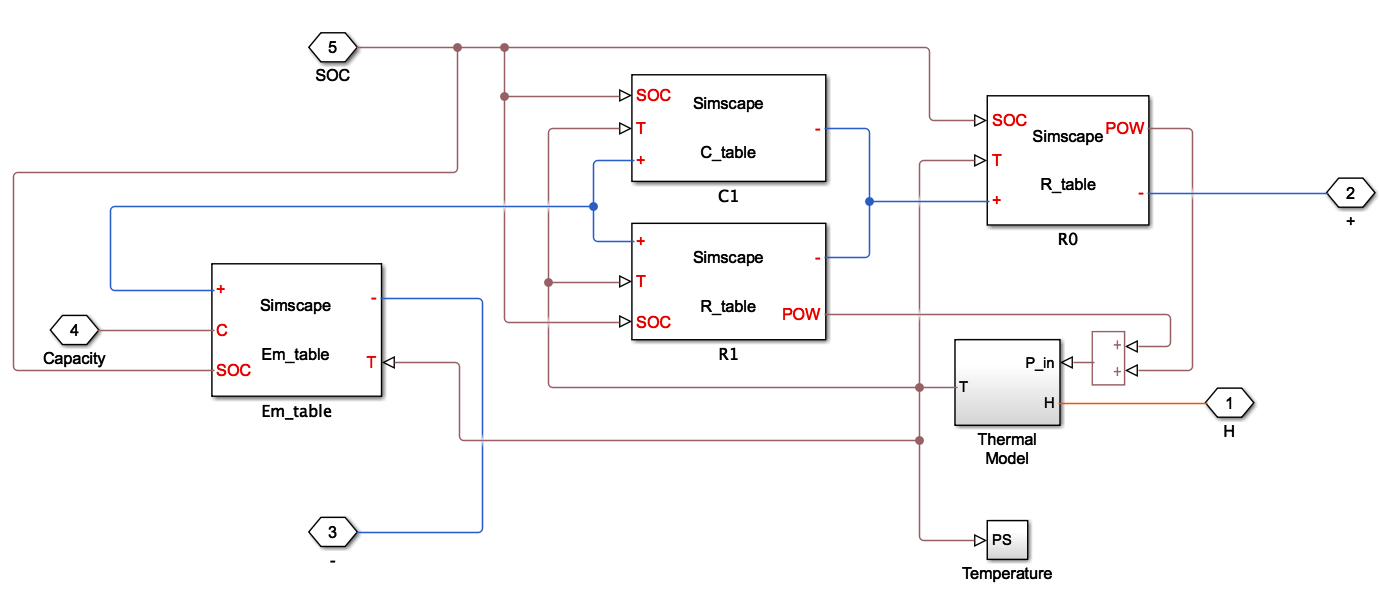
\includegraphics[height=2in, width=3in]{figures/BatteryModelSimscape}
\caption{Battery Model in Simscape}
\label{fig:battery_model_sim}
\end{figure}

\subsubsection{Battery Parameter Estimation}

The goal of battery parameter estimation is to estimate the value of $R_0$, $R_1$, $C_1$, and $Em$ in order to minimize the error between the experiment data and simulated data. In Figure \ref{fig:discharging_voltage_RW9}, the battery voltage of discharging cycle with a sequence of discharge current is given as the result of the experiment. 
With using known experiment data such as current and battery voltage, this parameter estimation technique will try to train the value of battery parameters so that the predicted voltage can mimic the real experiment data.

\begin{figure}
%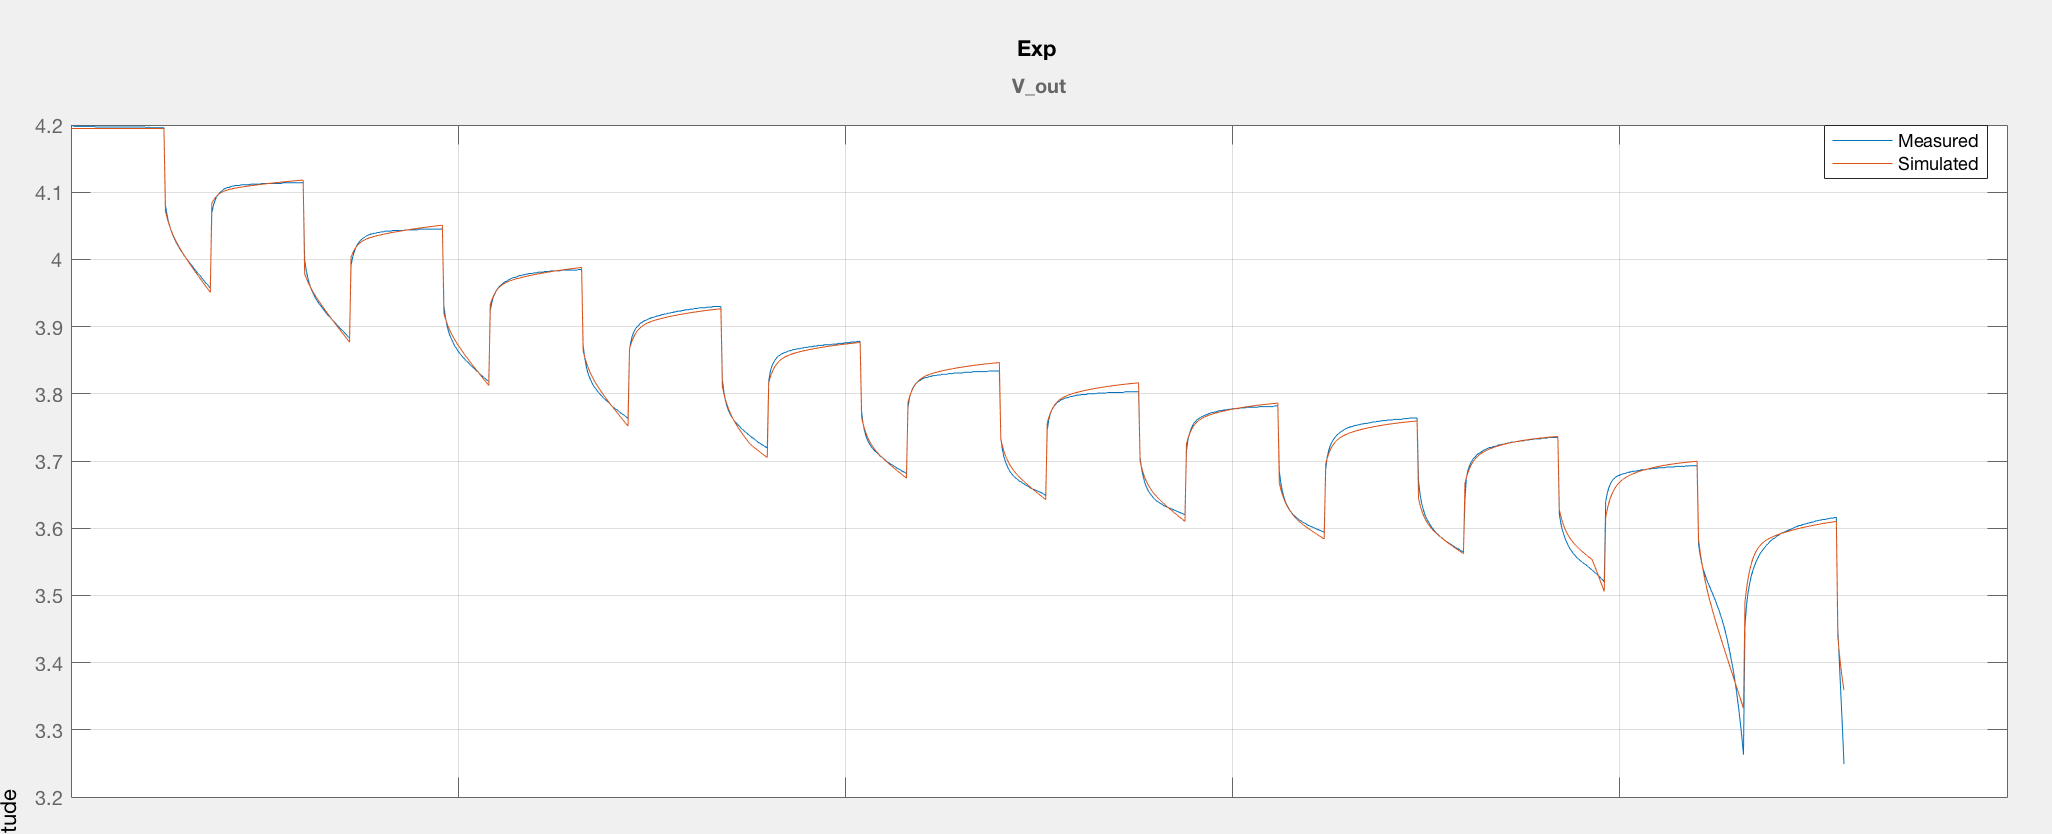
\includegraphics[height=3in, width=\textwidth]{figures/Discharging_01}
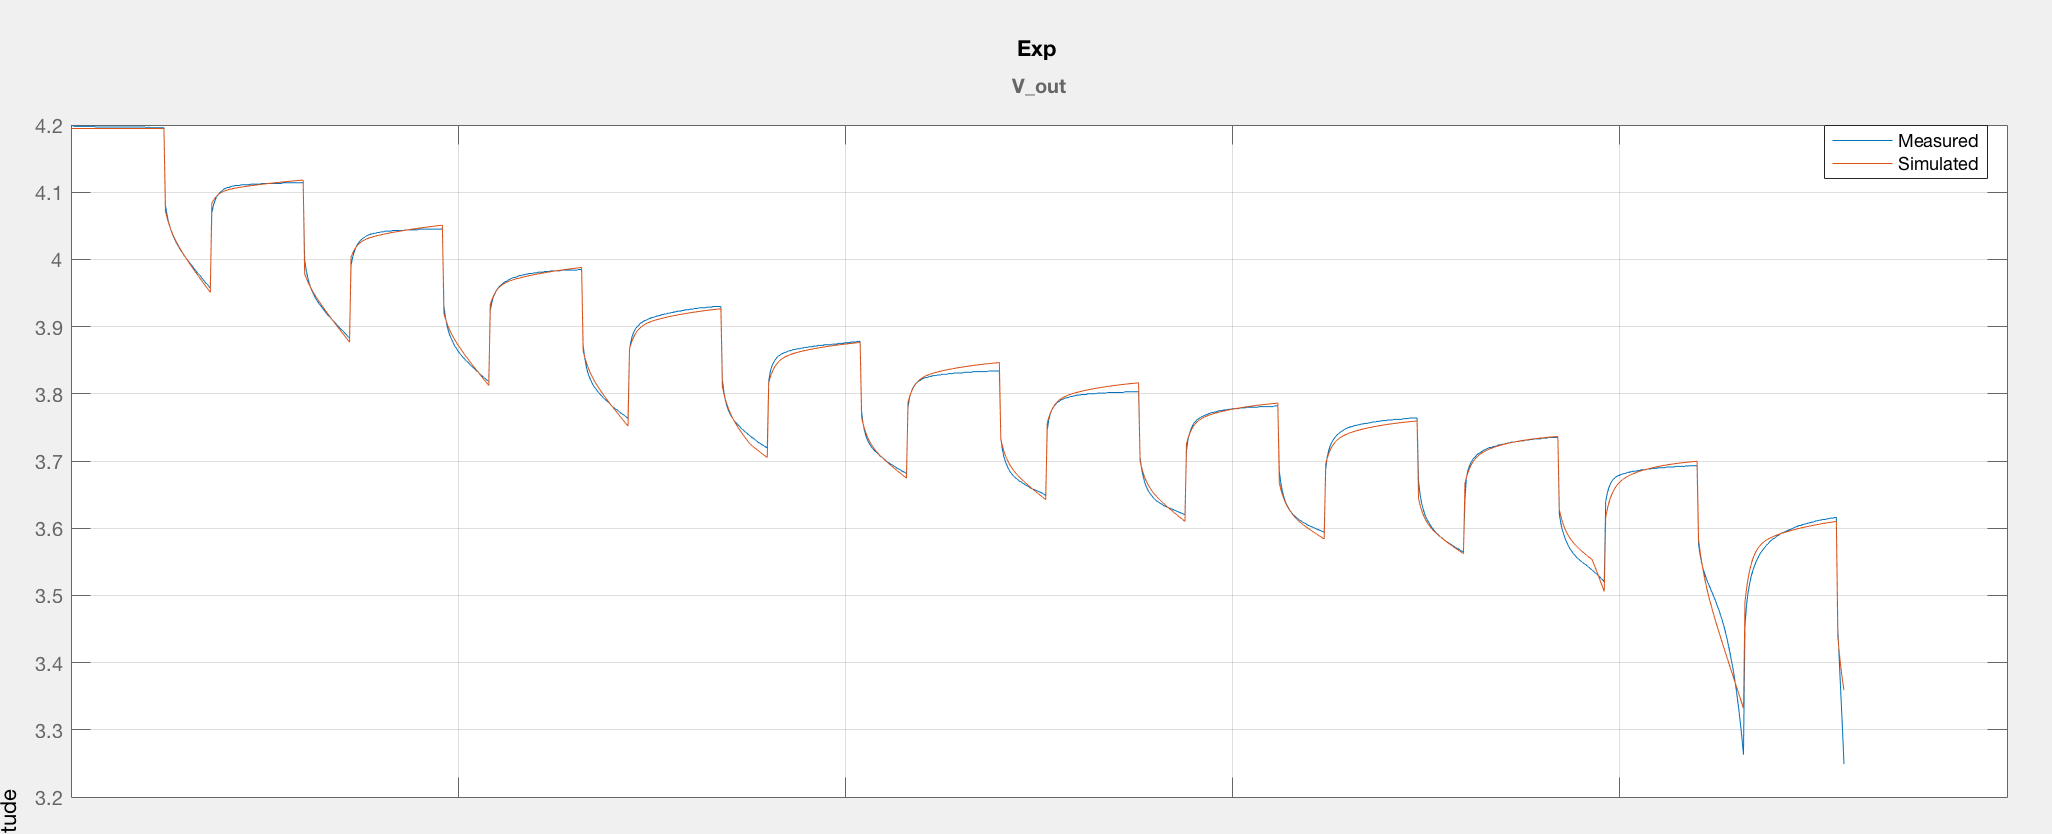
\includegraphics[height=1in, width=3in]{figures/Discharging_01}
\caption{Discharging Voltage of RW9}
\label{fig:discharging_voltage_RW9}
\end{figure}

As you can see on the Simulink Diagram in Figure \ref{fig:simulink_params}, we are going to feed current as the input of this simulation by using the current used in the real experiment. In addition, we also try to feed ambient temperature as another input for the battery to simulate its internal thermal condition. Later on, the voltage measurement of the battery is conducted so that error between the simulation and the real dataset can be calculated.

\begin{figure}
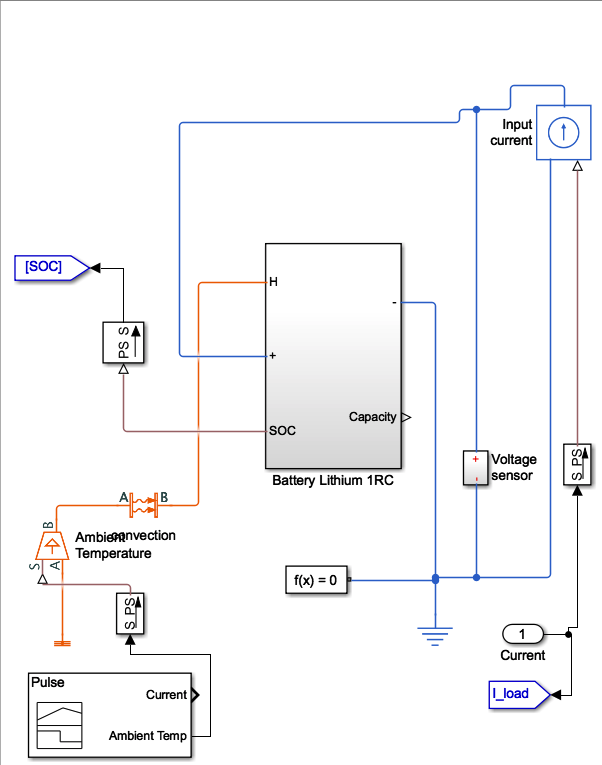
\includegraphics[height=3in, width=3in]{figures/Simulink_params}
\caption{Simulink diagram for parameter estimation}
\label{fig:simulink_params}
\end{figure}

\subsubsection{Kalman Filter and Battery Capacity Estimation}

Kalman Filtering is a common algorithm used in many applications including guidance and navigation of vehicles. It takes into account measures over time that might include noise and estimates future values based on its previous values.

To determine the remaining RUL of a battery, we use SOC and capacity of the battery. We followed the example\footnote{\url{https://www.mathworks.com/help/control/examples/nonlinear-state-estimation-of-a-degrading-battery-system.html}} provided in \cite{6183271} with the help of \MATLAB, Simulink and Simscape. The capacity of the battery degrades with every discharge-charge cycle, giving an inaccurate SOC estimation. Therefore, we can use an event-based linear Kalman filter to estimate the battery capacity when the battery transitions between charging and discharging. Consequently, we can use the estimated capacity to indicate the health condition of the battery (SOC).
\paragraph{Estimating SOC} From the previous Section  on the battery model, we can derive our state transition equation as below:
\begin{equation*}
  \label{state transition_1}
\begin{aligned}
\begin{split}
  \frac{d}{dt}  \left( \begin{array}{c} SOC \\ U_1 \end{array}\right) = \left( \begin{array}{c} 0 \\ - \frac{1}{R_1(SOC, T_b)*C_1(SOC, T_b)}U_1 \end{array}\right) + \\ \left( \begin{array}{c} -\frac{1}{3600*C_q} \\  \frac{1}{C_1(SOC, T_b)} \end{array}\right)I + W
 \end{split}
 \end{aligned}
\end{equation*}
where  $V_1$ is the voltage across capacitor $C_1$, $I$ is input current, $T_b$ is the battery temperature, $C_q$ is the battery capacity and $W$ is the process noise.

We will use Kalman Filtering to estimate the SOC of the battery with the help of Simulink functions. Since SOC is non-linear, we will use an Unscented Kalman Filter, details of which can be found in \cite{6183271} and \cite{882463}.

Applying Euler discretization of the state transition equation will give us:

\begin{equation*}
  \label{state transition_2}
\begin{aligned}
\begin{split}
 \left( \begin{array}{c} SOC_{T+1} \\ U_{1_{T+1}}\end{array}\right) = 
 \left( \begin{array}{c} -\frac{1}{3600*C_q}I \\-\frac{1}{R_1(SOC, T_b)*C_1(SOC, T_b)}U_1 + \frac{1}{C_1(SOC, T_b)}I\end{array}\right)T_s + \\
 + \left( \begin{array}{c} SOC_{T} \\ U_{1_{T}}\end{array}\right) + W_T
 \end{split}
 \end{aligned}
\end{equation*}
where $T_s$ is the sampling time.
The Kalman filter can be configured in Simulink, details of which can be found in \cite{6183271}.

\paragraph{Estimating Battery Capacity}
The decreasing capacity $Cq$ of the battery models the battery degradation. The battery is configured to charge when its capacity is at 30\% and discharge when it is at 90\%. Thus the measurement equations can be derived as:
\begin{equation}
  \label{measurement_equation}
\begin{aligned}
\begin{split}
 C_{q_k}^{measured} = C_{q_{k}} + V_{C_{q}} =  \frac{\int_{t_{k-1}}^{t_{k}}Idt} {(\Delta SOC)_{nominal}} = \\ = \frac{\int_{t_{k-1}}^{t_{k}}Idt} {\left|0.9 - 0.3 \right|} = \frac{\int_{t_{k-1}}^{t_{k}}Idt} {0.6}
 \end{split}
 \end{aligned}
\end{equation}
where $I$ is the input current.

The state transition and measurement equations are shown below:
\begin{itemize}
\item State Transition: 
	\begin{center}
	$C_{q_{k+1}} = C_{q_{k}} + W_{C_{q}}$
	\end{center}
\item Measurement Equation: 
\begin{center}
 $C_{q_k}^{measured} = C_{C{q}}C_{q_{k}} + V_{C_{q}}$
\end{center}
\end{itemize}

where $W_{C_q}$ is the process noise, $V_{C_q}$ is the measurement noise, $A_{C_q}$ and $C_{C_q}$ are constants that are set to 1.

\section{Results}
\subsection{Gaussian Process Regression}

The best GPR model created has a $RMSE$ of 0.1058, where voltage ranges from 4.2V to 3.2V, and uses an exponential kernel function.  The trained model performs well on both the train and test set, with almost the entire training (RW9) and testing (RW10) dataset falling inside the 95\% confidence bounds of the trained GPR model’s predictions.  An interesting characteristic of the model to note is that the predicted peaks are lower and the dips are higher than the actual values as shown in Figures \ref{fig:first_5k_rw9_v_model} to \ref{fig:last_5k_rw10_v_model}.
\begin{figure*}
\begin{multicols}{2}
	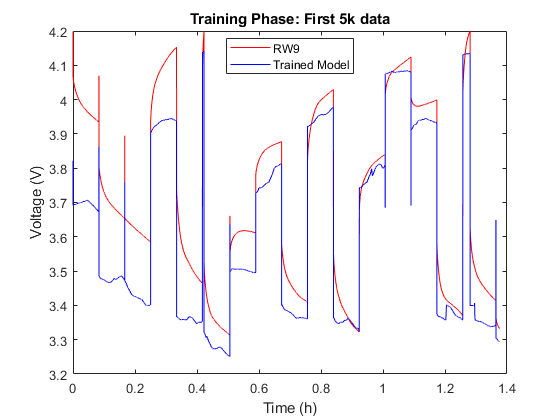
\includegraphics[height=2.3in, width=3.5in]{figures/GPR/first_5k_rw9_v_model}
	\caption{GPR Model: First 5K data of Model vs. Training Set (RW9)}
	\label{fig:first_5k_rw9_v_model}
	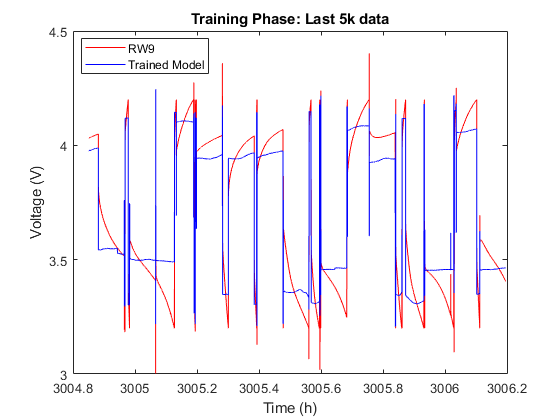
\includegraphics[height=2.3in, width=3.5in]{figures/GPR/last_5k_rw9_v_model}
	\caption{GPR Model: Last 5k data of Model vs. Training Set (RW9)}
	\label{fig:last_5k_rw9_v_model}
\end{multicols}
\begin{multicols}{2}
	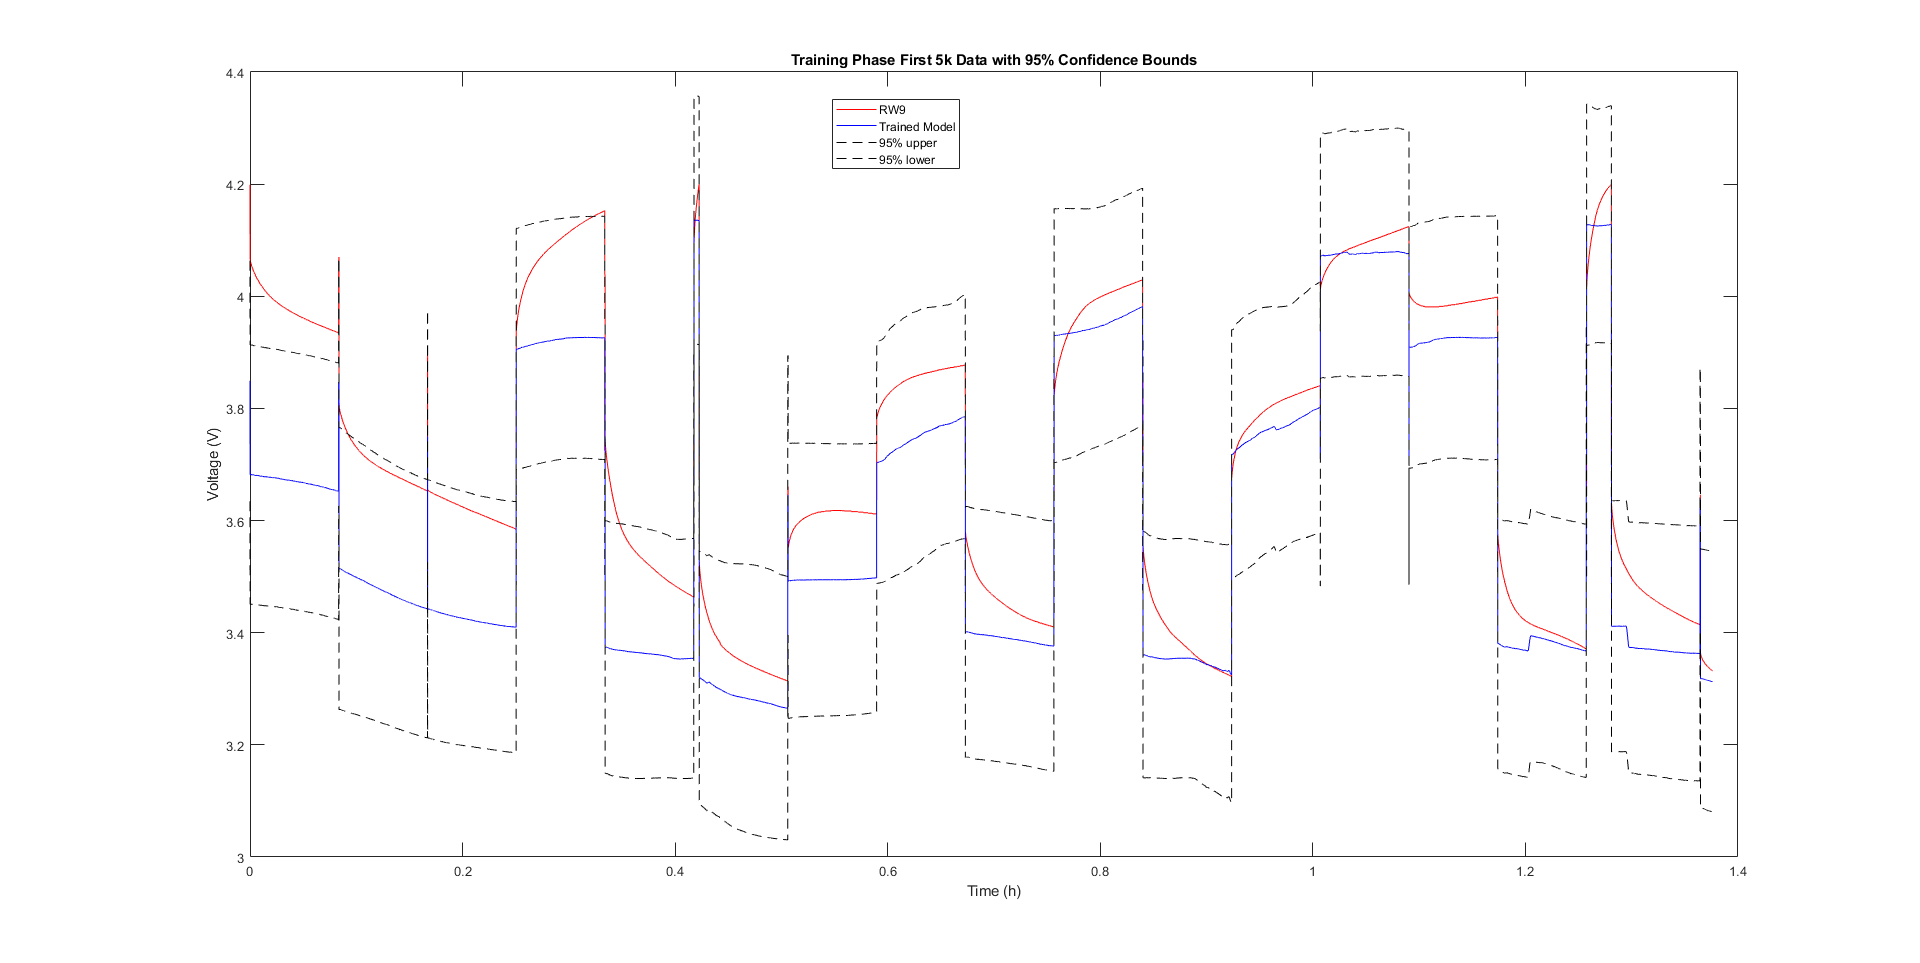
\includegraphics[height=2.3in, width=3.5in]{figures/GPR/first_5k_rw9_v_model_w_bounds}
	\caption{GPR Model: First 5K data of Model vs. Training Set (RW9) with 95\% conf bounds}
	\label{fig:first_5k_rw9_v_model_w_bounds}
	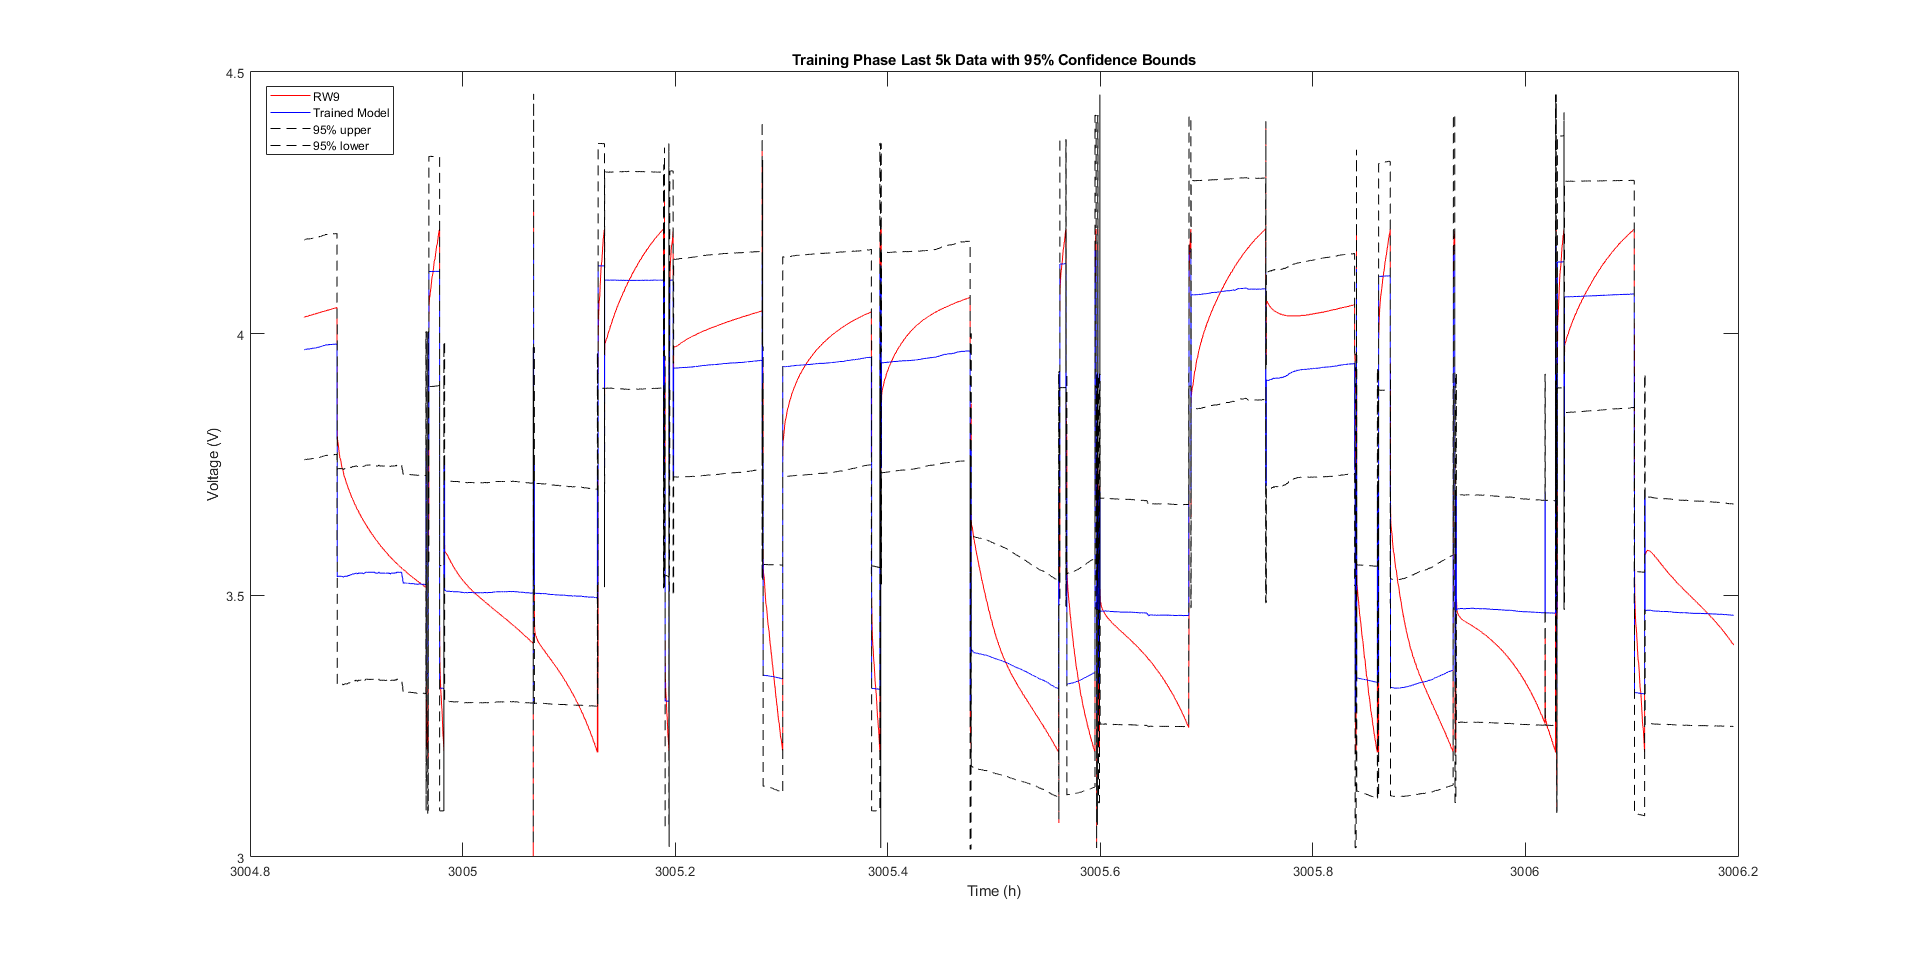
\includegraphics[height=2.3in, width=3.5in]{figures/GPR/last_5k_rw9_v_model_w_bounds}
	\caption{GPR Model: Last 5k data of Model vs. Training Set (RW9) with 95\% conf bounds}
	\label{fig:last_5k_rw9_v_model_w_bounds}
\end{multicols}
\begin{multicols}{2}
	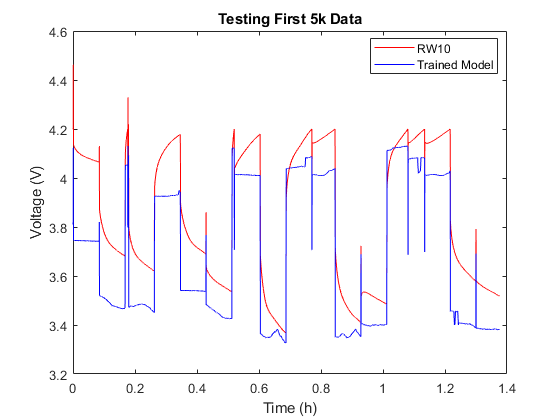
\includegraphics[height=2.3in, width=3.5in]{figures/GPR/first_5k_rw10_v_model}
	\caption{GPR Model: First 5K data of Model vs. Test Set (RW10)}
	\label{fig:first_5k_rw10_v_model}
	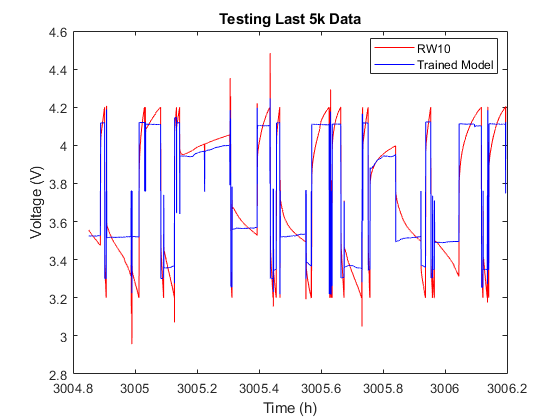
\includegraphics[height=2.3in, width=3.5in]{figures/GPR/last_5k_rw10_v_model}
	\caption{GPR Model: Last 5K data of Model vs. Test Set (RW10)}
	\label{fig:last_5k_rw10_v_model}
\end{multicols}
\end{figure*}
\begin{figure*}
\begin{multicols}{2}
	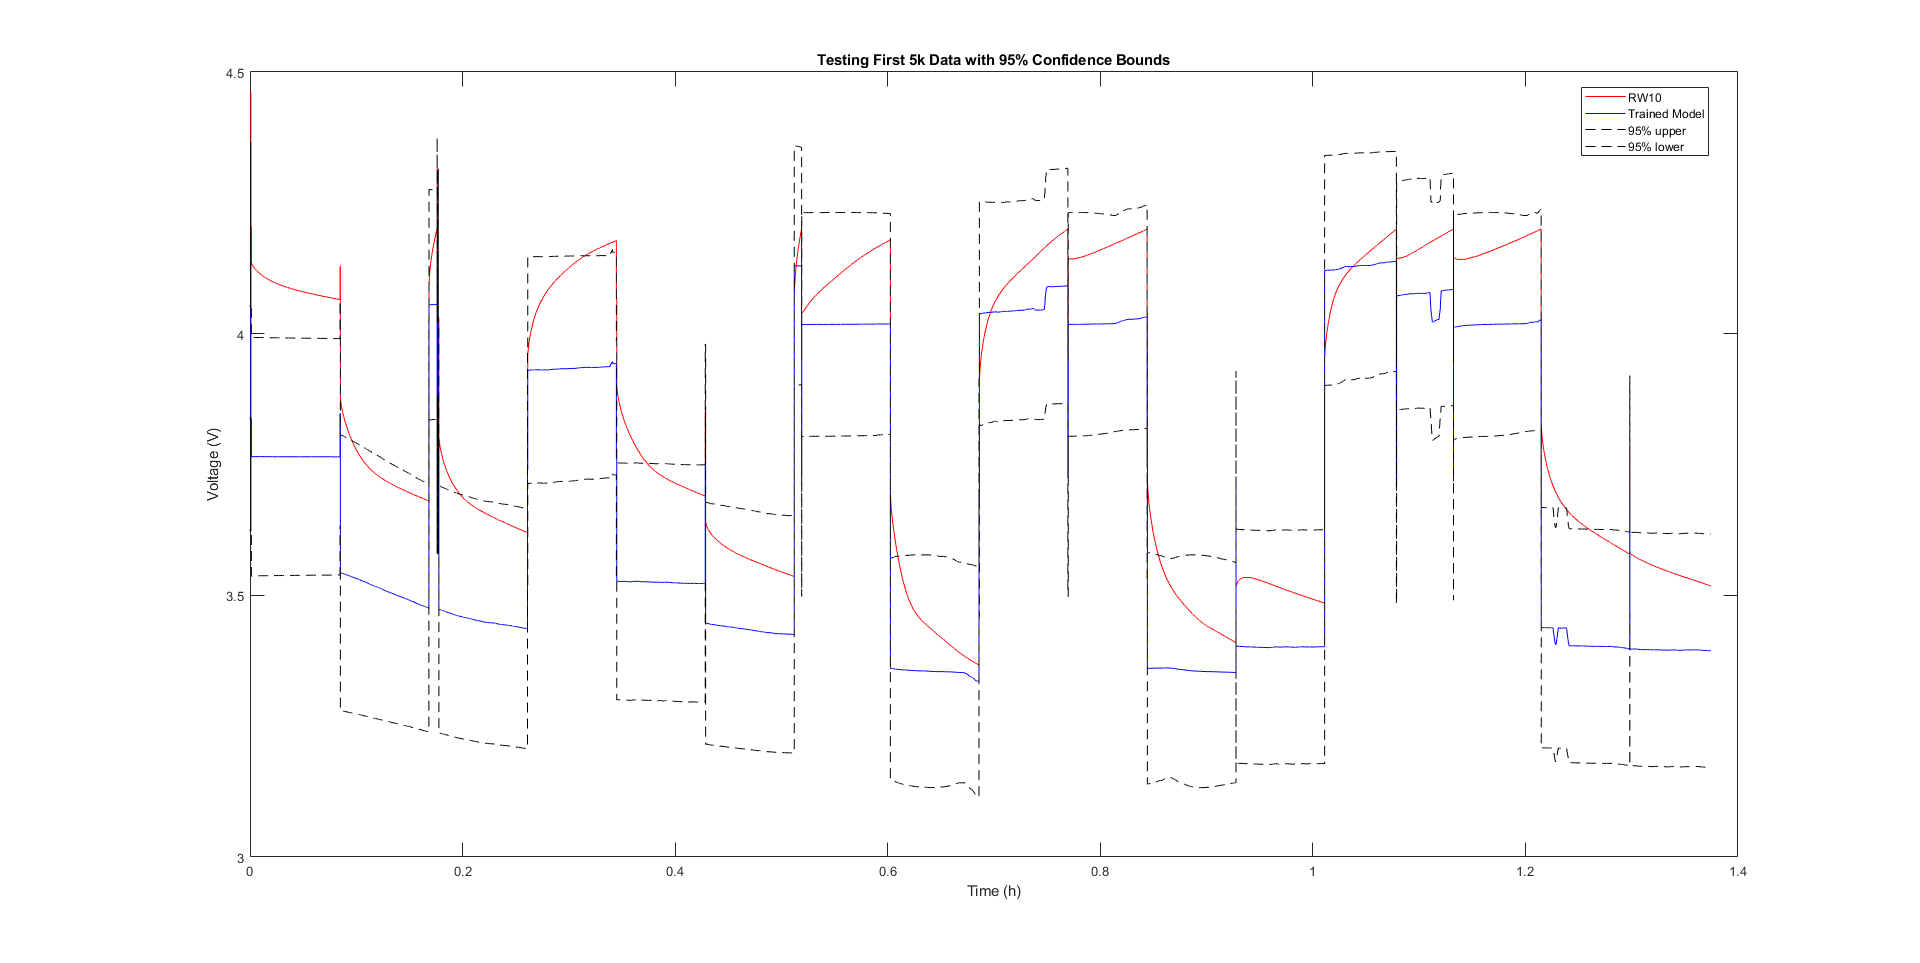
\includegraphics[height=2.3in, width=3.5in]{figures/GPR/first_5k_rw10_v_model_w_bounds}
	\caption{GPR Model: First 5K data of Model vs. Training Set (RW10) with 95\% conf bounds}
	\label{fig:first_5k_rw10_v_model_w_bounds}
	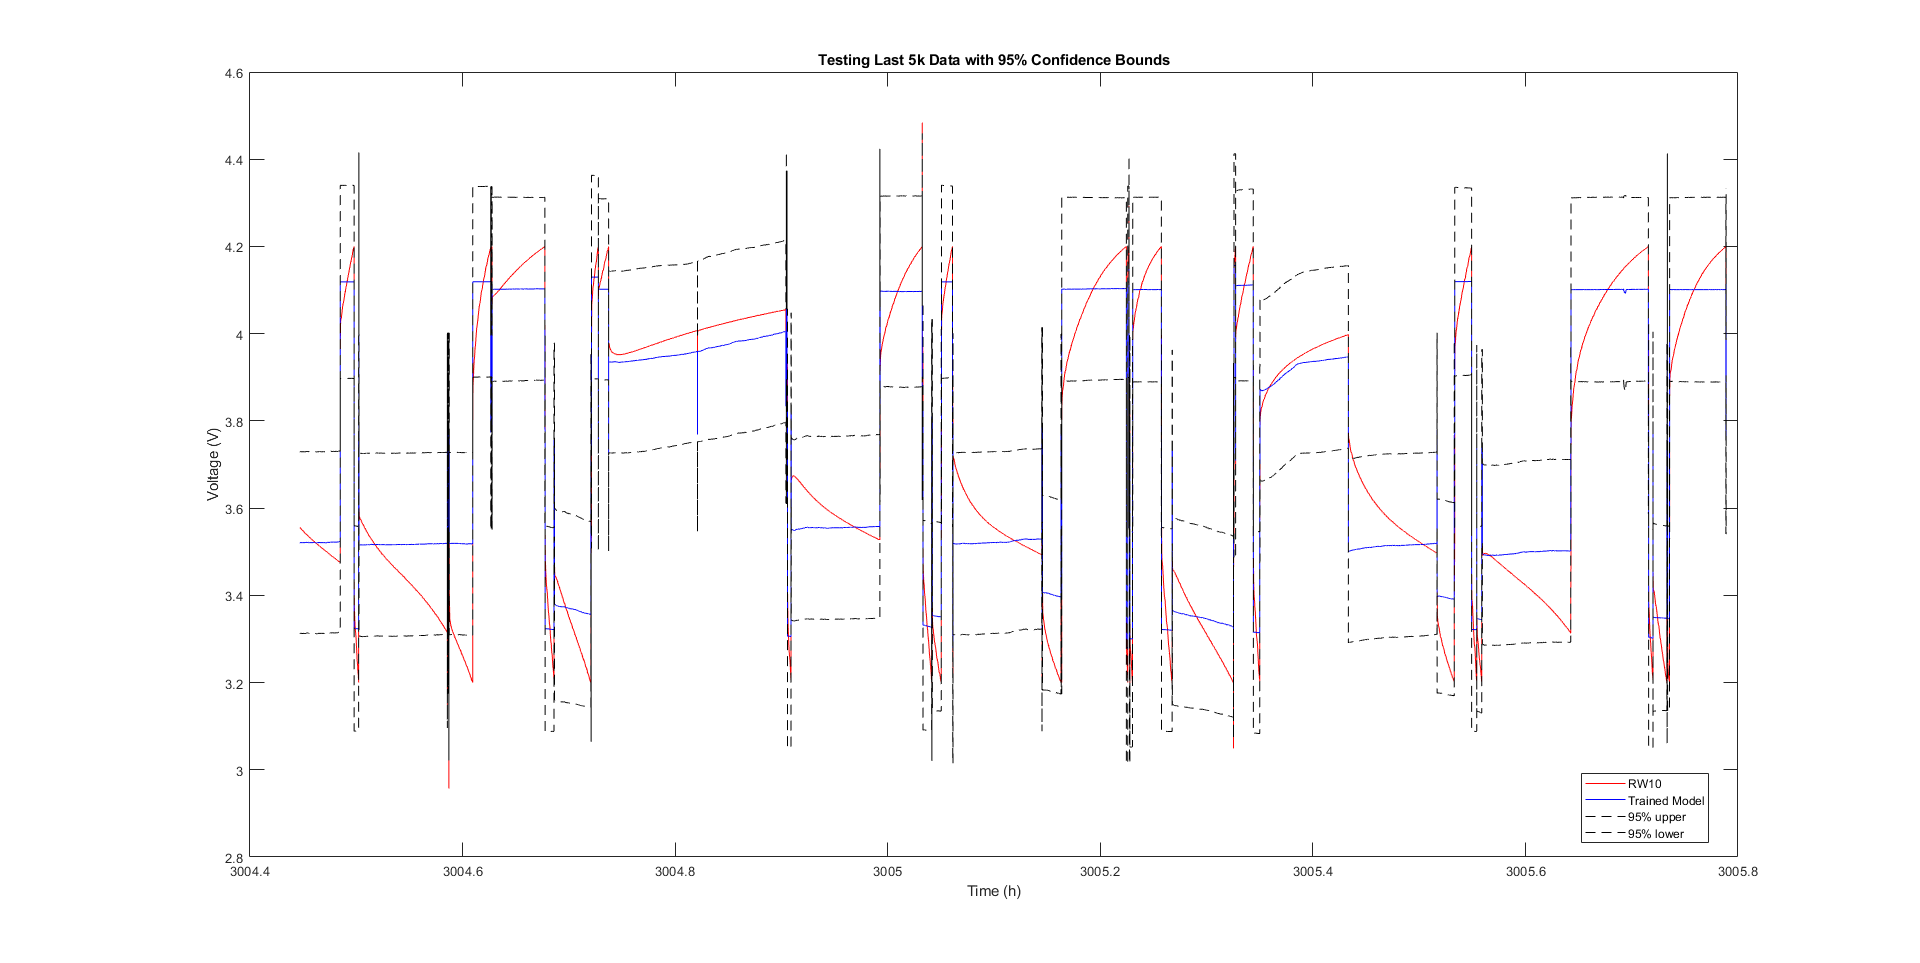
\includegraphics[height=2.3in, width=3.5in]{figures/GPR/last_5k_rw10_v_model_w_bounds}
	\caption{GPR Model:Last 5K data of Model vs. Training Set (RW10) with 95\% conf bounds}
	\label{fig:last_5k_rw10_v_model_w_bounds}
	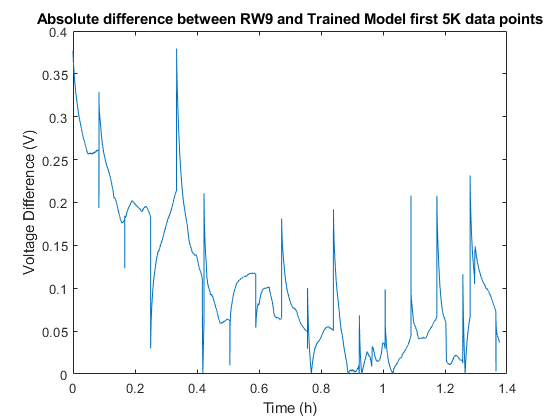
\includegraphics[height=2.3in, width=3.5in]{figures/GPR/first_5k_rw9_abs_v_diff}
	\caption{GPR Model: Absolute difference between RW9 and GPR model for first 5K data points}
	\label{fig:first_5k_rw9_abs_v_diff}
	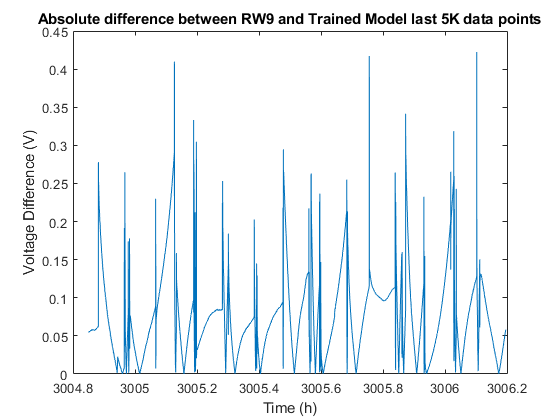
\includegraphics[height=2.3in, width=3.5in]{figures/GPR/last_5k_rw9_abs_v_diff}
	\caption{GPR Model: Absolute difference between RW9 and GPR model for last 5K data points}
	\label{fig:last_5k_rw9_abs_v_diff}
		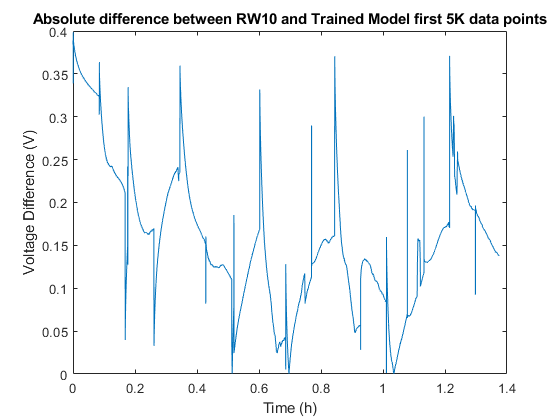
\includegraphics[height=2.3in, width=3.5in]{figures/GPR/first_5k_rw10_abs_v_diff}
	\caption{GPR Model: Absolute difference between RW10 and GPR model for first 5K data points}
	\label{fig:first_5k_rw10_abs_v_diff}
	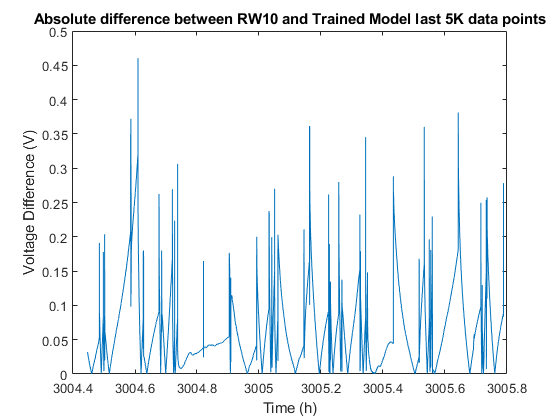
\includegraphics[height=2.3in, width=3.5in]{figures/GPR/last_5k_rw10_abs_v_diff}
	\caption{GPR Model: Absolute difference between RW10 and GPR model for last 5K data points}
	\label{fig:last_5k_rw10_abs_v_diff}
\end{multicols}
\end{figure*}

The error in the trained model’s prediction, measured as the absolute difference in voltage as shown in Figures \ref{fig:first_5k_rw9_abs_v_diff} to \ref{fig:last_5k_rw10_abs_v_diff}, against both the training and test data does not go down in time, rather it remains constant throughout the life of the battery.  However, the average error is quite low, only 0.0772V against the train set (RW9) and 0.0777V against the test set (RW10).  The similar error between the training and testing set is a good implication that the trained model is not overfitted.

\begin{figure*}
\begin{multicols}{2}
	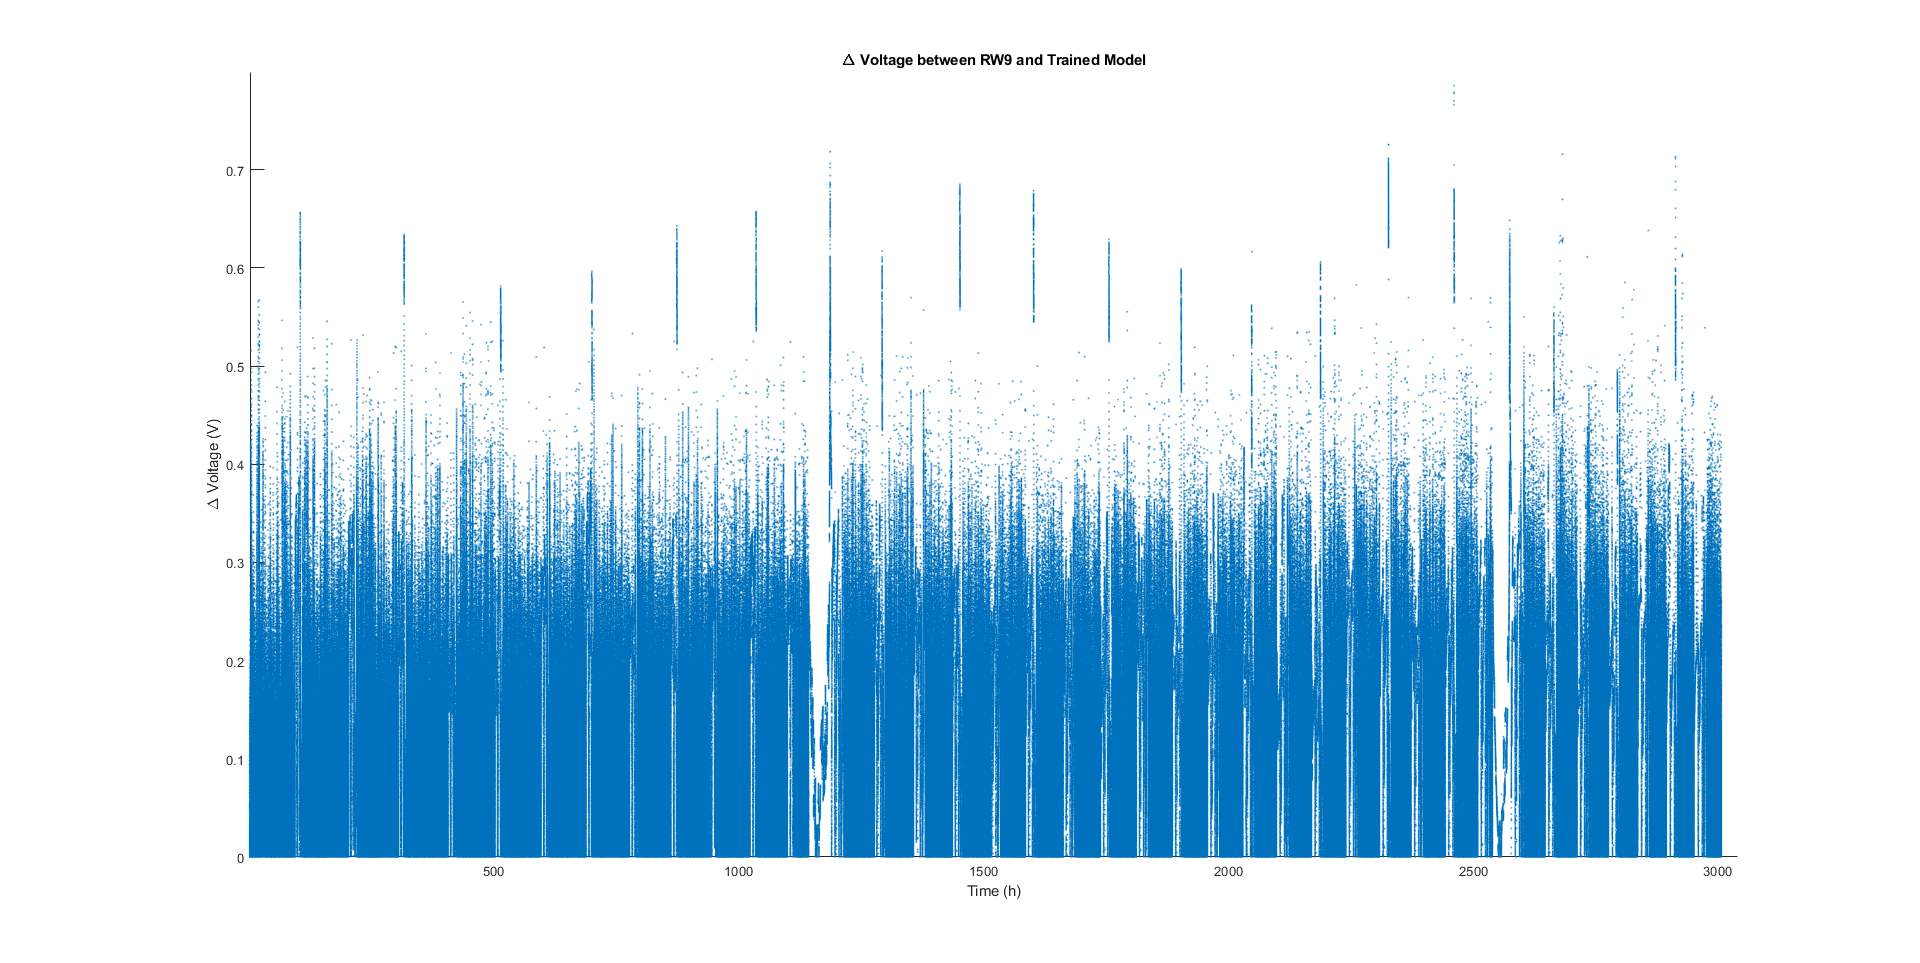
\includegraphics[height=2in, width=3in]{figures/GPR/rw9_abs_v_diff}
	\caption{GPR Model: Scatter Plot of Absolute difference between RW9 and GPR model}
	\label{fig:rw9_abs_v_diff}
	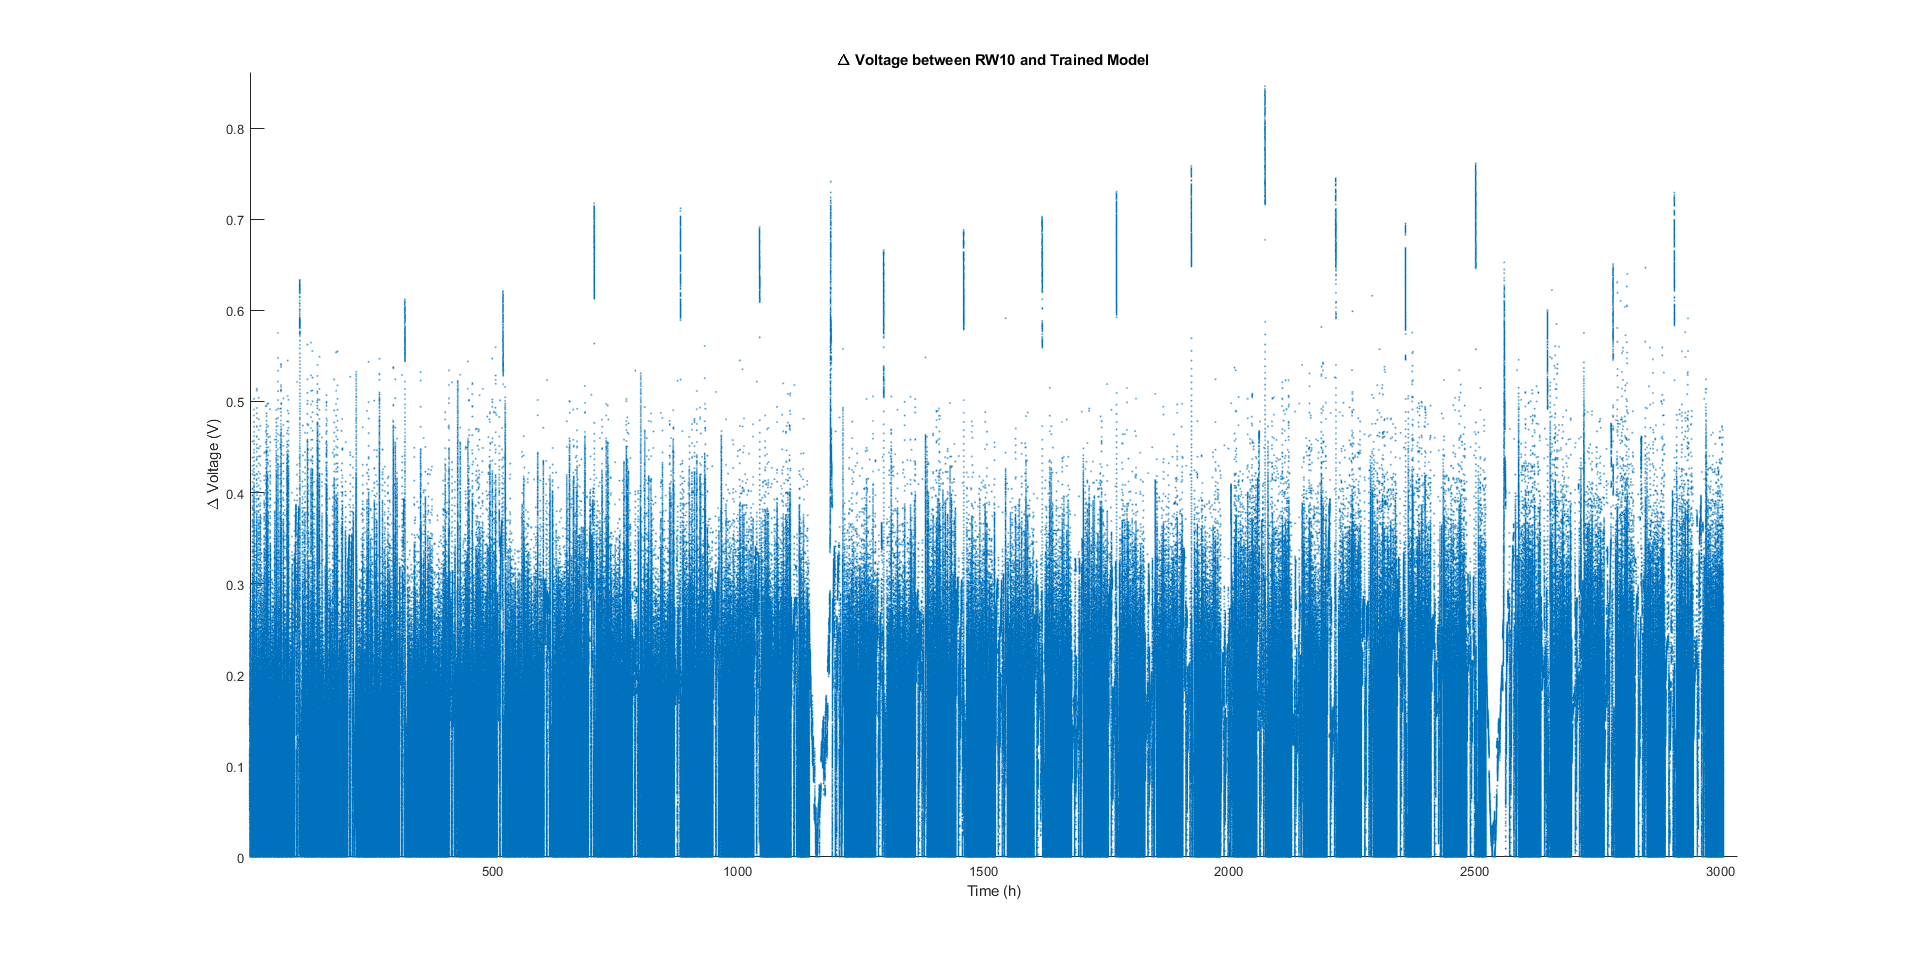
\includegraphics[height=2in, width=3in]{figures/GPR/rw10_abs_v_diff}
	\caption{GPR Model: Scatter Plot of Absolute difference between RW10 and GPR model}
	\label{fig:rw10_abs_v_diff}
\end{multicols}
\end{figure*}

Despite the ability for the GPR model to predict the state of the battery with relatively high predictive power, there are issues with how the model predicts future data that makes it impractical for prognostics.  Due to the fact that temperature and current are used as inputs along with time, if the model is at time $t$ and needs to predict voltage for $t+1$, the model requires the current and temperature at $t+1$ to be able to predict voltage at $t+1$.  This is obviously impractical to use for an alarm system as the future current and temperature is unknown to the model until it is measured at $t+1$, but at that point there is no value added to predict voltage for $t+1$, as it has already occurred and can be measured.

\subsection{Battery Modeling Using Battery Equivalent Circuit}

\subsubsection{Battery Parameter Estimation}

The simulated battery voltage of the battery with the initial parameter values is shown in Figure \ref{fig:simulation} . These initial values are manually chosen so that the transient state of the simulated data is close to the transient state of the real experiment. This setup is necessary in order to optimize the training efficiency. If the incorrect initial values are chosen, the parameter training could take more than 50 iterations to converge. Otherwise, it would take less than 10 iterations to reach at a converging point.

\begin{figure}
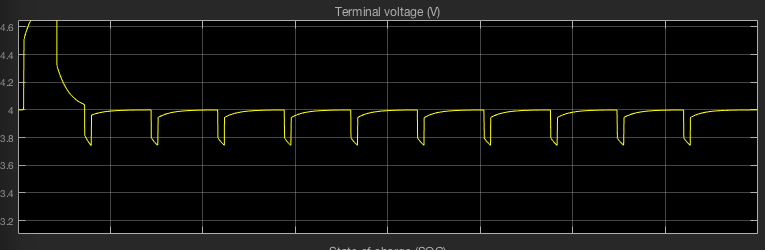
\includegraphics[height=1in, width=3in]{figures/Simulation}
\caption{Simulated data of battery Voltage using initial parameters value}
\label{fig:simulation}
\end{figure}

Figure \ref{fig:simMeasured} shows the simulation result after we successfully estimated the values of battery internal components. As shown on the image below, the measured and simulated lines are almost overlapped because the error of the simulation is quite small.

\begin{figure}
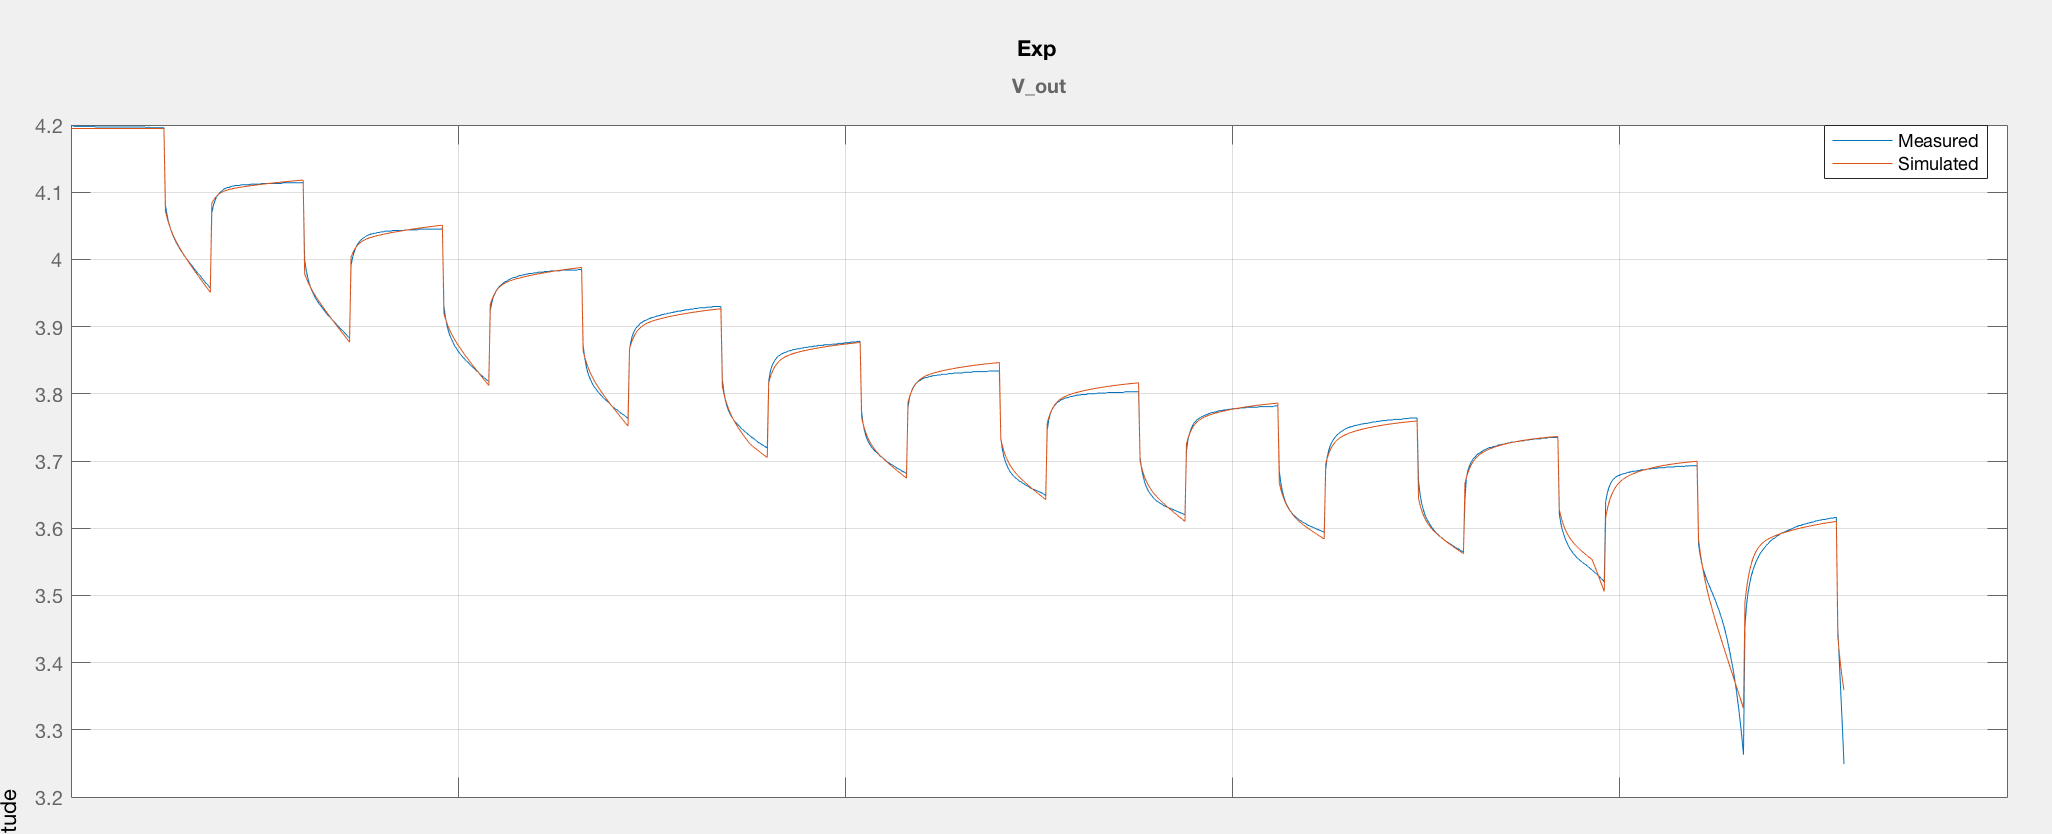
\includegraphics[height=1in, width=3in]{figures/SimMeasures}
\caption{Simulated and Measured Voltage of the experiments using trained parameters value}
\label{fig:simMeasured}
\end{figure}


As shown in Figure \ref{fig:iterations}, the value of $C_1$ is changing over the iteration during the parameter training until it converges. In addition, when the iteration is completed, we obtain the following results as the parameter values:
 \begin{equation*}

E_m=
  \begin{bmatrix}
    4 & 3.5917 & 3.1752 \\
    4 & 3.7324 & 3.5411 \\
    4 & 3.7794 & 3.6231 \\
    4 & 3.8961 & 3.7661 \\
    4 & 4.1431 & 3.9838 \\
    4 & 4.2894 & 4.0639 \\
    4 & 4.3648 & 4
  \end{bmatrix}
C_1=
  \begin{bmatrix}
    1000 & 9385 & 10308 \\
    1000 & 10139 & 10224 \\
    1000 & 12506 & 11170 \\
    1000 & 11854 & 10517 \\
    1000 & 12403 & 96195 \\
    1000 & 10945 & 94656 \\
    1000 & 10623 & 10000
  \end{bmatrix}
  
 \\
  R_1=
  \begin{bmatrix}
    0.07 & 0.0769 & 0.0712 \\
    0.07 & 0.0655 & 0.0641 \\
    0.07 & 0.0562 & 0.0626 \\
    0.07 & 0.0654 & 0.05697 \\
    0.07 & 0.0753 & 0.0738 \\
    0.07 & 0.0723 & 0.0732 \\
    0.07 & 0.0700 & 0.07
  \end{bmatrix}
  R_0=
  \begin{bmatrix}
    0.1 & 0.1297 & 0.1091 \\
    0.1 & 0.1024 & 0.0940 \\
    0.1 & 0.1035 & 0.0998 \\
    0.1 & 0.1039 & 0.1043 \\
    0.1 & 0.1087 & 0.0977 \\
    0.1 & 0.1006 & 0.1011 \\
    0.1 & 0.100 & 0.1
  \end{bmatrix}
 \end{equation*}
 
\begin{figure}
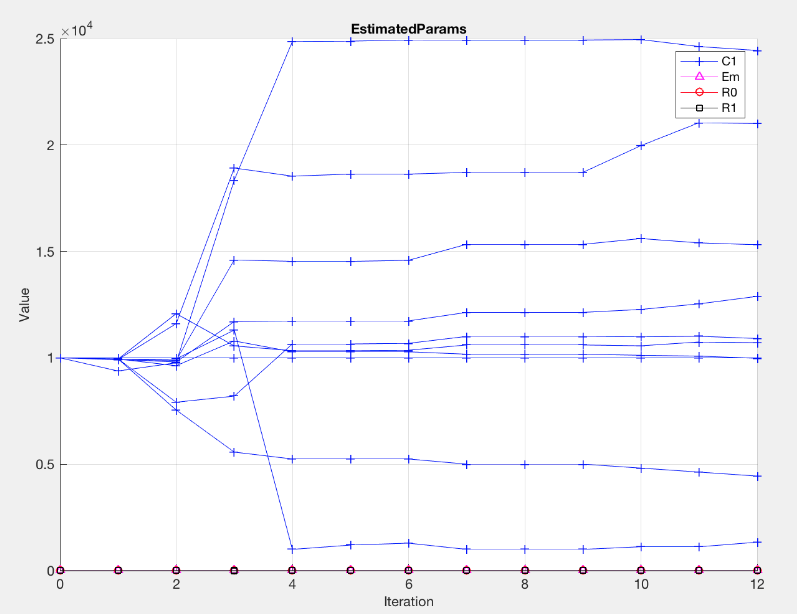
\includegraphics[height=2in, width=3in]{figures/Iterations}
\caption{Changes of parameters during training per iterations}
\label{fig:iterations}
\end{figure}

Later on, these parameter values of the battery will be used to estimate the SOC of the battery and the remaining useful capacity of the battery.

\subsubsection{Kalman Filter and Battery Capacity Estimation}
Performing Kalman Filtering on SOC and capacity produced the results shown in Figures \ref{fig:capacity_1} and \ref{fig:capacity_2}.
\begin{figure}
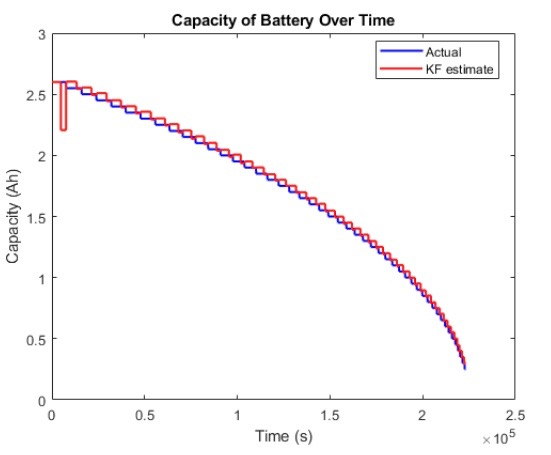
\includegraphics[height=2in, width=3in]{figures/capacity_1}
\caption{Actual and Estimated Capacity of Battery over time}
\label{fig:capacity_1}
\end{figure}
It is important to observe that the capacity of the battery decreases as the battery runs out of charge with time. It is also important to note that the actual capacity and estimated capacity are similar. There is a slight lag between the actual and estimated values, which is due to how the capacity is calculated, in that, we require the previous value of the capacity to estimate the next.
\begin{figure}
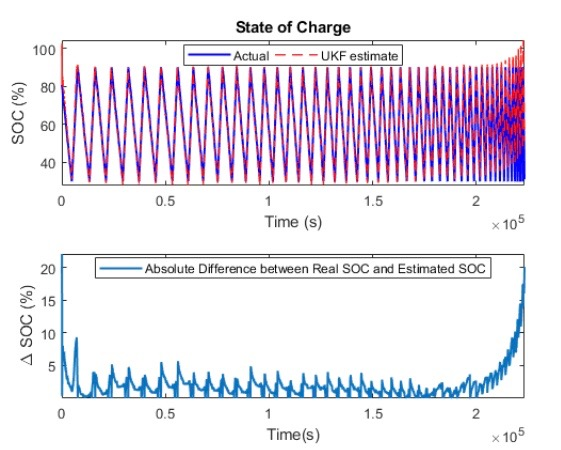
\includegraphics[height=2in, width=3in]{figures/capacity_2}
\caption{Actual and Estimated SOC with time}
\label{fig:capacity_2}
\end{figure}
In Figure \ref{fig:capacity_2}, it can be seen that as the battery discharges, the frequency of the SOC pattern increases. This means that it takes less time for the battery to charge and discharge, which supports our results from the Figure \ref{fig:capacity_1}. Note that because of this decrease in charging and discharging time, our estimates for SOC begin showing increased error as the sample rate is greater than the reduced charging/discharge time.

\section{Conclusion}
In conclusion, both the GPR and State Space Modeling of the battery can be used to predict the RUL of the battery. However there are tradeoffs between these methods. 

The GPR predicts the voltage battery with a relatively small error. However, this method shows serious time and space complexity limitations as it is slow to train ( approx. 1 hour) and can accept only a limited training set (less than 1\% of available data points). It also requires the inputs of the next time step to predict the output, and thus a usable alarm cannot easily be built.
The State Space Model of the Physical battery predicts the state of the battery through simulation. It is faster to train( approx.20 mins). It is shown to produce, with high accuracy, estimates of SOC and capacity. An alarm system can also be built using the fact that the charging or discharging time decreases as the battery state degrades.

\section{Future Work}
As of future work, the authors plan to further investigate the capabilities of Gaussian Process Regression (GPR) so that the model will not require future inputs to predict future outputs, but will aim to predict each individual feature using temperature as an alternative output feature. Moreover, the goal is to construct an alarm system that will leverage the results obtained from the Kalman Filtering approach : using the estimated capacity curve and the measured State of Charge behavior of the battery, an alarm will be triggered when the required recharge period drops below a certain threshold, indicating deteriorating capacity.

 
 
